% Software Frontend (HTML/CSS/JS; Vue.js)
% Zuständig: Arthur

\section{Software - Frontend}
\label{sec:software_frontend}
Das Frontend ist eine Webseite und dient zur Visualisierung der gesammelten Daten vom Server.
Darunter zählen die Daten vom LiDAR-Sensor, vom Beschleunigungssensor und die Geschwindigkeit der Roboter
mithilfe der Encoder. Um das ganze geschehen der Roboter mitverfolgen zu können, ohne hinterherrennen zu müssen
werden auch die Kamerabilder der unterschiedlichen Roboter angezeigt.

Das Frontend wird mithilfe von Vue.js programmiert. Vue.js ist ein JavaScript Framework und bietet 
verschiedene Möglichkeiten, an die Webseite zu programmieren. Bei Vue.js kann man zwischen den Möglichkeiten "Options" und "Composition" unterscheiden.
Das Verhalten des Codes bleibt gleich, bietet aber eine andere Syntax. Der große Vorteil des Vue.js Frameworks ist, dass es einem bietet 
HTML, CSS und JavaScript in eine sogenannte "SFC"\footnote{Single-File Components} einzubinden. Durch eine SFC schreibt man HTML, CSS und JavaScript in einer Datei, anstatt in vielen unterschiedlichen
Dateien, die alle zueinander finden müssen.  

\subsection{LiDAR-Karte}
\label{subsec:frontend_lidar_map}
Die LiDAR-Karte wird mithilfe von Vue.js auf dem Frontend, der Webseite generiert und soll Hindernisse wie Wände, Säulen oder auch Menschen mit farbigen Punkten anzeigen. 
Neben der verschiedenen Hindernisse, die auf der Karte einzusehen sind, sollen auch die Position der Roboter markiert werden. 
\begin{figure}[H]
    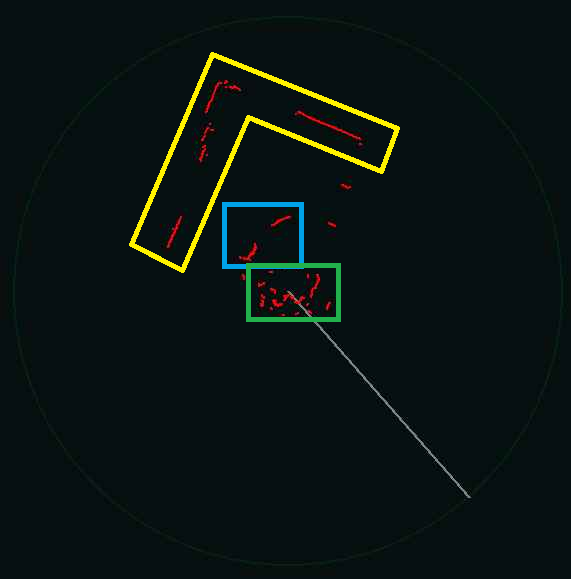
\includegraphics[width=0.4\textwidth, center]{img/LiDARMessungZeichnung_alt.png}
    \caption{LiDAR-Messung}
    \label{fig:LiDAR-Messung}
\end{figure}
Das Bild zeigt die generierte Punktwolke des LiDAR-Sensors. Die Punktwolke zeigt ideal die Funktionsweise des LiDARs und ist leicht zu interpretieren. 
Die unterschiedlichen Laserimpulse, welche gesendet werden, reflektieren an der Oberfläche und werden gemessen. Nicht nur ist die Entfernung, sondern auch die Tiefenwahrnehmung somit feststellbar.

Um die Punktwolke genauer zu verstehen, wurden Sektionen eingezeichnet. 
Die Grüne Sektion zeigt Objekte, welche unmittelbar vor dem LiDAR standen, in dem Fall waren es Büromaterialien wie etwa Kugelschreiber, Hefte, etc.
Die blaue Sektion befindet sich ca. 1-2 m vom LiDAR entfernt. Die aufgenommenen Punkte sind einfach nur eine Person sowie ein Sessel.
Die gelbe Sektion war ca. 3 m entfernt und zeigt die Umrandung des Raumes, interessanterweise sind die Lücken die Fenster, wo die Laserimpulse nicht reflektiert worden sind
und somit konnten keine Punkte an der Stelle der Wolke generiert werden konnten.

\subsection{Fernüberwachung per Kamera}
\label{subsec:frontend_cam_stream}
Auf allen drei Robotern befinden sich fest montierte ESP32-Kameras zur Überwachung, welche auf dem Frontend, der Webseite gestreamet werden.
Die Kameras dienen vor allem nur der Überwachung der Roboter und sollen der Gruppe nur helfen, Gefahren rechtzeitig zu identifizieren, um die Sicherheit des Projektes zu gewährleisten. Eingriffe erfolgen nur sofern die Roboter nicht selbst auf die Gefahr reagieren.
Sollte jedoch ein Fehler bei einem Roboter unterlaufen sein, so können wir mithilfe der Fernsteuerung (Siehe Abschnitt \ref{subsec:frontend_control}) probieren, die Roboter aus der Gefahrenzone zu entfernen.

\subsection{Fernsteuerung}
\label{subsec:frontend_control}
Die Idee der Fernsteuerung wurde aus den Prototypen der Projektwoche aus dem Jahr 2023/2024 übernommen. Diese hatten eine Fernsteuerungsfunktion, die hier in der Diplomarbeit nur in Notfällen oder Testzwecken verwendet wird.  

\subsection{Anzeigen der Sensordaten}
\label{subsec:frontend_sensors}
Die Sensordaten werden alle auf dem Frontend dargestellt und stetig aktualisiert. Die Sensoren, welche die Gruppe verwendet, sind der LiDAR, die Beschleunigungssensoren und die Kompasse.
Der LiDAR erstellt eine Karte mithilfe von einer Punktwolke, um die Hindernisse und Entfernungen feststellen zu können. Für mehr Informationen siehe Abschnitt \ref{subsec:frontend_lidar_map}.
%TODO BILD ÄNDERN
\begin{figure}[H]
    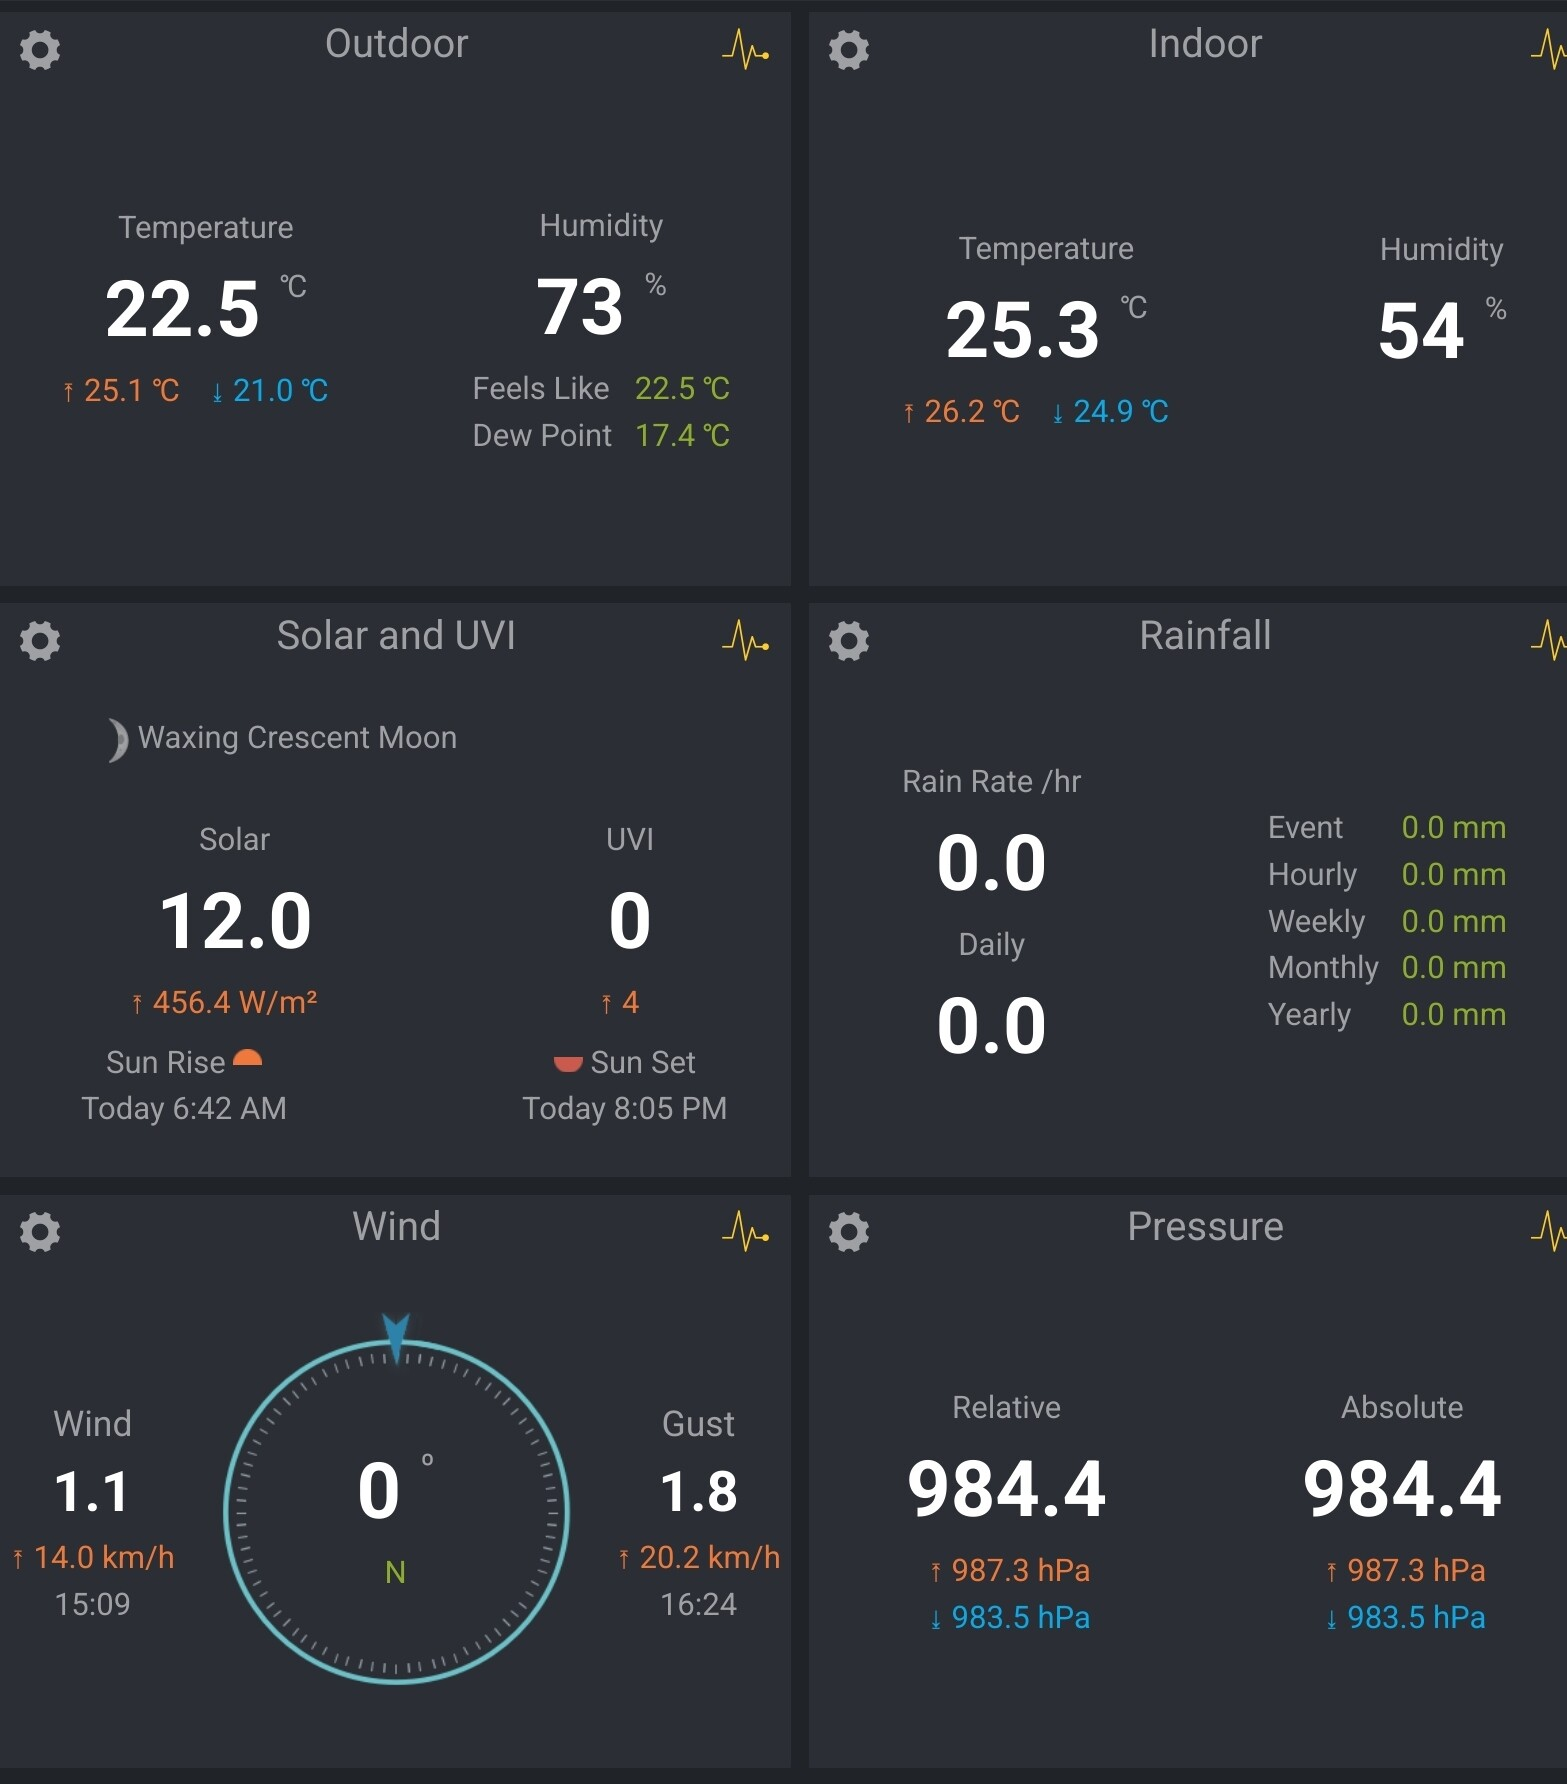
\includegraphics[width=0.4\textwidth, center]{img/Sensor_Anzeige_LOESCHEN.png}
    \caption{Anzeige der Sensordaten}
    \label{fig:Sensordaten}
\end{figure}
Die Beschleunigungssensoren werden in Graphen abhängig von der Zeit angezeigt, um die aktuellen Werte mit den vergangenen Werten vergleichen zu können. Nicht nur werden die Werte in Graphen abgebildet, sondern auch "normal" als Dezimalzahl
um schnell den aktuellsten Wert lesen zu können.
\\
Die Kompasse zeigen die aktuelle Fahrtrichtung der Roboter an. Geplant ist ein "realer" 2D-Kompass, wo die jedoch die Nadel die Fahrtrichtung anzeigt, statt wie gewohnt den Norden.